\section{Вступ}

Голосова взаємодія --- важливий аспект життя кожної людини. Автоматизація цієї голосової взаємодії інтенсивно розвивається, особливо в таких галузях як робототехніка \cite{Ishiguro_2016}, інтернет речей (ІОТ) та у зв’язку з автоматизацію багатьох процесів, зокрема у транспорті \cite{Kravchenko_2009,Heisterkamp_2001} та дистрибуції  \cite{art2,conf9}. Запровадження голосових інтерфейсів допомагає звільнити руки від управління технічними пристроями та зробити цей процес більш зручним і природним для людини.

Формалізація голосової взаємодії є достатньо важливим напрямом. У більшості систем це досягається переведенням голосової інформації у текст з подальшим використанням. Такий підхід є достатньо розповсюдженим і існує велика кількість готових систем розпізнавання голосу у текст, але для забезпечення високої якості, такі системи потребують великої кількості ресурсів, тому зазвичай вони встановлюються на серверах, а для їх використання необхідний постійний доступ до мережі інтернет для зв’язку з ними. Крім того, для використання систем формалізації голосової інформації в автоматизованих системах управління недостатньо перевести голосову інформацію в текст, необхідно ще забезпечити виділення керуючого впливу з отриманої команди.

Існують системи голосового управління, які не потребують розпізнавання голосової інформації і перетворення її в текстову форму, а можуть одразу визначити керуючий вплив з вимовленої команди. Так наприклад, рефлекторні системи голосового управління \cite{Egorchenkov_2016,Teslia_2014,Teslia_2013} на основі теорії несилової взаємодії \cite{Teslia_2010} працюють за таким принципом і складаються з двох основних частин: фонемного стенографа \cite{Pylypenko_2008}, який перетворює звуковий запис на фонемну репрезентацію, і ядра класифікації, яке визначає зміст та керуючий вплив з отриманого набору фонем.

Для автоматизації голосової взаємодії можуть бути використані певні заздалегідь створені сценарії голосової взаємодії \cite{art3}, які допоможуть системі визначити зміст сказаного. Створення подібних сценаріїв взаємодії має сенс для технологічних ситуацій, в яких взаємодія відбувається за певним протоколом, наприклад, у промислових системах, перемовинах з диспетчерами в різних галузях: медицина, авіація \cite{Korsun_2013}, правоохоронні органи чи дистрибуція \cite{art3}. Створення сценаріїв голосової взаємодії для вільного спілкування людей не має наразі настільки важливого економічного значення, але такі спроби теж існують, наприклад для подолання сором’язливості \cite{Ishiguro_2016}.

Центральна ланка формалізації голосової взаємодії — це класифікація вимовлених команд серед заздалегідь створених можливих сценаріїв взаємодії. Для виконання цієї класифікації можуть бути використані різні методи машинного навчання.

\section{Мета роботи}

Мета статті полягає у порівнянні ефективності методів машинного навчання для формалізації голосової взаємодії на прикладі системи підтримки диспетчеризації автотранспорту з використанням рефлекторної системи голосового управління.

\section{Викладення основного матеріалу}

Рефлекторні системи голосового управління складаються з двох основних частин: фонемного стенографа \cite{Pylypenko_2008}, який перетворює звуковий запис на фонемну репрезентацію, і ядра класифікації, яке визначає зміст та керуючий вплив кожного з отриманих наборів фонем. У якості ядра класифікації було запропоновано дуальну систему класифікації фонемної репрезентації голосових команд \cite{art4}, яка може використовувати метод інтелектуальних рефлекторних систем (ІРС) \cite{Egorchenkov_2016} або метод згорткових нейронних мереж (ЗНМ) для різних предметних областей, в залежності від того, який показує кращі результати.

Згорткові нейронні мережі для роботи з фонемами найбільше нагадують використання методу згорткових нейронних мереж для задачі класифікації текстів \cite{Kim_2014}, але оперують з «текстом» не за словами, а пофонемно, що схоже на роботу з текстом посимвольно \cite{Zhang_2015}.

Була розроблена модель голосової взаємодії водія та системи підтримки диспетчеризації автотранспорту у вигляді дерева сценаріїв \cite{art4}, яка складається з з 64 основних команд (реакцій) та поділяє всю множину голосової взаємодії на 19 контекстів, що можуть бути змодельовані окремо.

З метою перевірки ефективності побудованих моделей було проведено ітеративний процес збору даних та моделювання, який передбачав аналіз отриманих результатів та введення нових критеріїв оцінки, якщо попередні не давали достатньої точності оцінювання. У цілому цей процес апробації засобів формалізації голосової інформації в системах диспетчерського контролю за рухом автотранспорту можна розбити на два основні етапи.

На першому етапі була зібрана широка вибірка голосових даних згідно із моделлю дерева сценаріїв голосової взаємодії в системах підтримки диспетчеризації автотранспорту. Зібрані голосові дані можна охарактеризувати наступними параметрами:

\begin{itemize}
	\item 4 пристрої, 23 диктори (11 жінок, 12 чоловіків), 94 варіанти стимулів (64 на основні реакції), 3046 зразків;
	\item додатково 23 варіанти стимулів та 465 голосових зразків для реакції розпізнавання часу.
\end{itemize}

Детальний розподіл голосових даних, зібраних на першому етапі моделювання, представлено в таблиці \ref{tbl:data1_distribution}. Ця таблиця показує розподіл зібраних голосових зразків за пристроями та дикторами, а також повідомляє загальну кількість голосових зразків надиктованих кожним диктором, кількість унікальних реакцій та варіантів формулювання стимулів різними словами серед зібраних голосових зразків. В окрему колонку виведено кількість додаткових записів для реакції розпізнавання часу.

\begin{mytable}[ht]{ | c | c | c | c | c | c | c | }%
	{Детальний розподіл за дикторами та пристроями голосових даних зібраних на першому етапі моделювання}%
	{\label{tbl:data1_distribution}}%
	{
		\specialcellrot{3cm}{Диктор} & 
		\specialcellrot{3cm}{Пристрій} & 
		\specialcellrot{3cm}{Стать} & 
		\specialcellrot{3cm}{Кількість \\ записів} & 
		\specialcellrot{3cm}{Кількість \\ реакцій} &
		\specialcellrot{3cm}{Кількість варі-\\антів стимулів} & 
		\specialcellrot{3cm}{Кількість запи-\\сів реакції часу}}
	
	1 & 1 & жін. & 109 & 64 & 92 & 22 \\
	\hline
	2 & 1 & жін. & 105 & 64 & 96 & 22 \\
	\hline
	3 & 1 & жін. & 100 & 64 & 96 & 21 \\
	\hline
	4 & 1 & жін. & 97 & 64 & 93 & 22 \\
	\hline
	5 & 1 & жін. & 96 & 64 & 93 & 22 \\
	\hline
	6 & 1 & жін. & 95 & 64 & 94 & 22 \\
	\hline
	7 & 1 & жін. & 95 & 64 & 95 & 23 \\
	\hline
	8 & 1 & жін. & 95 & 62 & 90 & 21 \\
	\hline
	9 & 1 & жін. & 90 & 62 & 89 & 22 \\
	\hline
	10 & 1 & жін. & 79 & 58 & 79 & 23 \\
	\hline
	11 & 1 & чол. & 196 & 64 & 96 & 44 \\
	\hline
	12 & 1 & чол. & 101 & 64 & 94 & 25 \\
	\hline
	13 & 1 & чол. & 96 & 64 & 92 & 22 \\
	\hline
	14 & 1 & чол. & 98 & 63 & 95 & 21 \\
	\hline
	15 & 1 & чол. & 89 & 63 & 85 & 22 \\
	\hline
	16 & 1 & чол. & 98 & 62 & 90 & 21 \\
	\hline
	17 & 1 & чол. & 64 & 48 & 62 & 22 \\
	\hline
	18 & 1 & чол. & 30 & 25 & 30 & 0 \\
	\hline
	19 & 1 & чол. & 23 & 16 & 22 & 0 \\
	\hline
	20 & 1 & чол. & 23 & 9 & 19 & 0 \\
	\hline
	21 & 2 & жін. & 97 & 64 & 94 & 22 \\
	\hline
	22 & 3 & чол. & 96 & 64 & 96 & 22 \\
	\hline
	23 & 4 & чол. & 99 & 64 & 96 & 24 \\
	
\end{mytable}%

Як можна бачити, не всі диктори надиктували повний перелік реакцій згідно до моделі голосової взаємодії в системах підтримки диспетчеризації. Це має сенс, оскільки не всі водії будуть стикатися з усіма можливими позаплановими подіями. Також деякі диктори надиктували повністю ідентичні фрази кілька разів, що б мати можливість виключити вплив сторонніх шумів і певної стохастичності вимови та запису звуку, а деякі диктори надиктували різні варіанти формулювання та вимови стимулів, що б мати можливість навчити систему виділяти ключову інформацію в різних формулюваннях природної мови.

Першим було проведене моделювання методом інтелектуальних рефлекторних систем з розміром N-грам 1–3. Результати моделювання наведено в таблиці \ref{tbl:total_data1_irs13}. Було створено окрему модель для кожного контексту взаємодії водія та системи підтримки диспетчеризації автотранспорту, а також модель розпізнавання реакцій для всієї вибірки, без використання контекстів. Крім контекстів, представлених у моделі голосової взаємодії, було використано додатковий тестовий контекст, який складався з трьох реакцій найпростішого дерева сценаріїв голосової взаємодії \cite{art3}.

\begin{mytable}[ht]{ | c | c | c | c | c | c | }%
	{Результати моделювання першого набору даних використовуючи ІРС з послідовностями розміром 1--3}%
	{\label{tbl:total_data1_irs13}}%
	{
		\specialcellrot{3cm}{№ Контексту} & 
		\specialcellrot{3cm}{Точність \\ розпізнання} & 
		\specialcellrot{3cm}{Середня \\ прецизійність} & 
		\specialcellrot{3cm}{Середня \\ повнота} & 
		\specialcellrot{3cm}{Середня \\ F-міра} & 
		\specialcellrot{3cm}{Кількість}}	
	
	1 & 0.677 & 0.450 & 0.445 & 0.447 & 124 \\
	\hline
	2 & 0.456 & 0.559 & 0.663 & 0.408 & 513 \\
	\hline
	3 & 0.387 & 0.055 & 0.143 & 0.080 & 217 \\
	\hline
	4 & 0.375 & 0.217 & 0.271 & 0.171 & 104 \\
	\hline
	5 & 0.339 & 0.108 & 0.184 & 0.111 & 183 \\
	\hline
	6 & 0.397 & 0.198 & 0.252 & 0.222 & 209 \\
	\hline
	7 & 0.206 & 0.021 & 0.098 & 0.034 & 233 \\
	\hline
	8 & 0.346 & 0.182 & 0.179 & 0.107 & 217 \\
	\hline
	9 & 0.344 & 0.144 & 0.225 & 0.141 & 131 \\
	\hline
	10 & 0.349 & 0.489 & 0.255 & 0.194 & 126 \\
	\hline
	11 & 0.268 & 0.099 & 0.145 & 0.114 & 239 \\
	\hline
	12 & 0.264 & 0.303 & 0.250 & 0.238 & 201 \\
	\hline
	13 & 0.450 & 0.361 & 0.259 & 0.182 & 171 \\
	\hline
	14 & 0.439 & 0.551 & 0.432 & 0.432 & 139 \\
	\hline
	15 & 0.302 & 0.547 & 0.210 & 0.152 & 159 \\
	\hline
	16 & 0.478 & 0.539 & 0.470 & 0.450 & 115 \\
	\hline
	17 & 0.271 & 0.261 & 0.263 & 0.248 & 155 \\
	\hline
	18 & 0.418 & 0.482 & 0.411 & 0.407 & 110 \\
	\hline
	19 & 0.471 & 0.650 & 0.458 & 0.462 & 87 \\
	\hline
	\specialcell{3cm}{По всій \\ вибірці} & 0.044 & 0.027 & 0.017 & 0.009 & 2069 \\
	\hline
	\specialcell{3cm}{Тестовий \\ контекст} & 0.485 & 0.162 & 0.333 & 0.218 & 101 \\
\end{mytable}

Розміри N-грам 1–3 було обрано, виходячи з того, що метод інтелектуальних рефлекторних систем має квадратичну залежність швидкості розрахунку від максимального розміру N-грам. З таблиці \ref{tbl:total_data1_irs13}  видно, що точність розпізнавання цих моделей не перевищує 50\% для жодного з контекстів, крім першого. Тому для підвищення якості моделей було проведено моделювання цим же методом, але з розміром N-грам 2–4. Результати цього моделювання представлено в таблиці \ref{tbl:total_data1_irs24}.

\begin{mytable}[ht]{ | c | c | c | c | c | c | }%
	{Результати моделювання першого набору даних використовуючи ІРС з послідовностями розміром 2--4}%
	{\label{tbl:total_data1_irs24}}%
	{
		\specialcellrot{3cm}{№ Контексту} & 
		\specialcellrot{3cm}{Точність \\ розпізнання} & 
		\specialcellrot{3cm}{Середня \\ прецизійність} & 
		\specialcellrot{3cm}{Середня \\ повнота} & 
		\specialcellrot{3cm}{Середня \\ F-міра} & 
		\specialcellrot{3cm}{Кількість}}		
	
	1 & 0.710 & 0.503 & 0.442 & 0.459 & 124 \\
	\hline
	2 & 0.895 & 0.465 & 0.478 & 0.471 & 513 \\
	\hline
	3 & 0.382 & 0.048 & 0.124 & 0.069 & 217 \\
	\hline
	4 & 0.558 & 0.740 & 0.480 & 0.484 & 104 \\
	\hline
	5 & 0.415 & 0.434 & 0.259 & 0.225 & 183 \\
	\hline
	6 & 0.565 & 0.282 & 0.359 & 0.316 & 209 \\
	\hline
	7 & 0.232 & 0.388 & 0.127 & 0.089 & 233 \\
	\hline
	8 & 0.373 & 0.410 & 0.207 & 0.157 & 217 \\
	\hline
	9 & 0.527 & 0.737 & 0.437 & 0.449 & 131 \\
	\hline
	10 & 0.532 & 0.773 & 0.468 & 0.486 & 126 \\
	\hline
	11 & 0.515 & 0.207 & 0.282 & 0.238 & 239 \\
	\hline
	12 & 0.488 & 0.510 & 0.469 & 0.452 & 201 \\
	\hline
	13 & 0.485 & 0.448 & 0.303 & 0.283 & 171 \\
	\hline
	14 & 0.633 & 0.703 & 0.625 & 0.625 & 139 \\
	\hline
	15 & 0.453 & 0.480 & 0.329 & 0.333 & 159 \\
	\hline
	16 & 0.583 & 0.661 & 0.574 & 0.550 & 115 \\
	\hline
	17 & 0.387 & 0.473 & 0.378 & 0.374 & 155 \\
	\hline
	18 & 0.582 & 0.672 & 0.576 & 0.583 & 110 \\
	\hline
	19 & 0.655 & 0.728 & 0.650 & 0.642 & 87 \\
	\hline
	\specialcell{3cm}{По всій \\ вибірці} & 0.122 & 0.061 & 0.048 & 0.027 & 2069 \\
	\hline
	\specialcell{3cm}{Тестовий \\ контекст} & 0.475 & 0.160 & 0.327 & 0.215 & 101 \\
\end{mytable}

Як альтернативний класифікатор у дуальній системі класифікації фонемної репрезентації голосових команд використано метод згорткових нейронних мереж \cite{art4}. На відміну від методу інтелектуальних рефлекторних систем, метод згорткових нейронних мереж залежить від розміру фільтрів лише лінійно, оскільки замість всіх можливих наборів N-грам, використовується лише певна фіксована кількість фільтрів, які навчаються методом зворотного розповсюдження помилки. Тому для моделювання методом згорткових нейронних мереж використовувалися лише фільтри розміром 2–4. Результати цього моделювання представлено в таблиці \ref{tbl:total_data1_cnn}.

\begin{mytable}[ht]{ | c | c | c | c | c | c | }%
	{Результати моделювання першого набору даних використовуючи ЗНМ з послідовностями розміром 2--4}%
	{\label{tbl:total_data1_cnn}}%
	{
		\specialcellrot{3cm}{№ Контексту} & 
		\specialcellrot{3cm}{Точність \\ розпізнання} & 
		\specialcellrot{3cm}{Середня \\ прецизійність} & 
		\specialcellrot{3cm}{Середня \\ повнота} & 
		\specialcellrot{3cm}{Середня \\ F-міра} & 
		\specialcellrot{3cm}{Кількість}}		
	
	1 & 0.879 & 0.880 & 0.863 & 0.870 & 124 \\
	\hline
	2 & 0.957 & 0.933 & 0.799 & 0.851 & 513 \\
	\hline
	3 & 0.820 & 0.870 & 0.777 & 0.813 & 217 \\
	\hline
	4 & 0.846 & 0.857 & 0.829 & 0.837 & 104 \\
	\hline
	5 & 0.798 & 0.814 & 0.734 & 0.754 & 183 \\
	\hline
	6 & 0.852 & 0.851 & 0.789 & 0.814 & 209 \\
	\hline
	7 & 0.785 & 0.808 & 0.773 & 0.785 & 233 \\
	\hline
	8 & 0.871 & 0.895 & 0.847 & 0.867 & 217 \\
	\hline
	9 & 0.863 & 0.871 & 0.836 & 0.847 & 131 \\
	\hline
	10 & 0.825 & 0.841 & 0.818 & 0.819 & 126 \\
	\hline
	11 & 0.908 & 0.922 & 0.850 & 0.878 & 239 \\
	\hline
	12 & 0.846 & 0.852 & 0.849 & 0.847 & 201 \\
	\hline
	13 & 0.848 & 0.860 & 0.842 & 0.849 & 171 \\
	\hline
	14 & 0.842 & 0.851 & 0.838 & 0.838 & 139 \\
	\hline
	15 & 0.849 & 0.842 & 0.829 & 0.834 & 159 \\
	\hline
	16 & 0.817 & 0.826 & 0.814 & 0.814 & 115 \\
	\hline
	17 & 0.723 & 0.729 & 0.723 & 0.720 & 155 \\
	\hline
	18 & 0.836 & 0.842 & 0.837 & 0.835 & 110 \\
	\hline
	19 & 0.862 & 0.871 & 0.863 & 0.856 & 87 \\
	\hline
	\specialcell{3cm}{По всій \\ вибірці} & 0.652 & 0.679 & 0.622 & 0.640 & 2069 \\
	\hline
	\specialcell{3cm}{Тестовий \\ контекст} & 0.891 & 0.915 & 0.871 & 0.888 & 101 \\
\end{mytable}

Таблиці \ref{tbl:total_data1_irs13}, \ref{tbl:total_data1_irs24} та \ref{tbl:total_data1_cnn} включають деякі міри оцінки якості моделей та кількість звукових записів, які використовувалися для навчання та оцінки моделей. Спочатку в якості основної міри використовувалася точність (accuracy) \cite{Ting_2011}, що може бути розрахована за наступною формулою:

\begin{equation}
\label{eq:acuracy}
A=\frac{\sum\limits_i TP_i}{\sum\limits_i TP_i+FN_i},
\end{equation}

де $A$ --- точність, $TP_i$ --- кількість вірно розпізнаних (True positive) зразків реакції $i$, a $FN_i$ --- кількість зразків реакції $i$, хибно розпізнаних (False negative) як інша реакція.

Оскільки частота реакцій у більшості контекстів не збалансована, точність може показувати кращі результати, ніж справжня якість моделі.

Побудувавши графіки розподілу точності та F-міри від кількості зразків у контексті (рис. \ref{img:accuracy_distribution_data1}) ми можемо бачити, що прямої залежності немає. Але на якість розпізнавання повинна впливати кількість реакцій в контексті і середня кількість записів зразків голосових даних на кожну реакцію.

\begin{figure}[!t]
	\centering
	\subbottom[Метод ІРС розміром 1--3 \label{img:accuracy_distribution_data1_irs13}]{%
		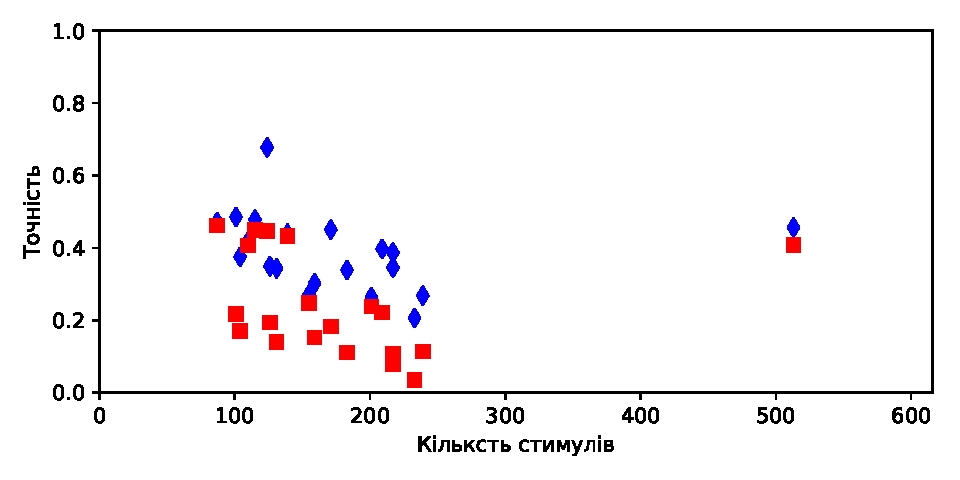
\includegraphics[width=\linewidth]{accuracy_distribution_data1_irs13}}
	\\
	\subbottom[Метод ІРС розміром 2--4 \label{img:accuracy_distribution_data1_irs24}]{%
		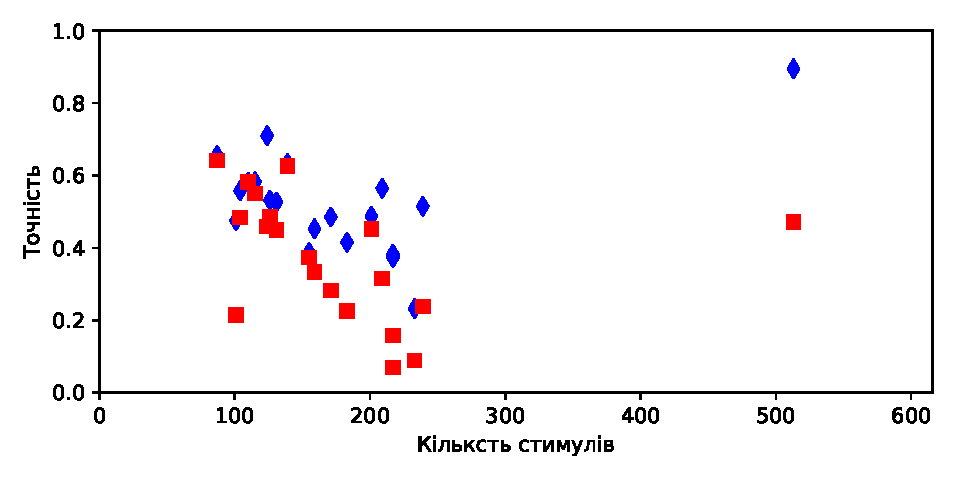
\includegraphics[width=\linewidth]{accuracy_distribution_data1_irs24}}
	\\
	\subbottom[Метод ЗНМ \label{img:accuracy_distribution_data1_cnn}]{%
		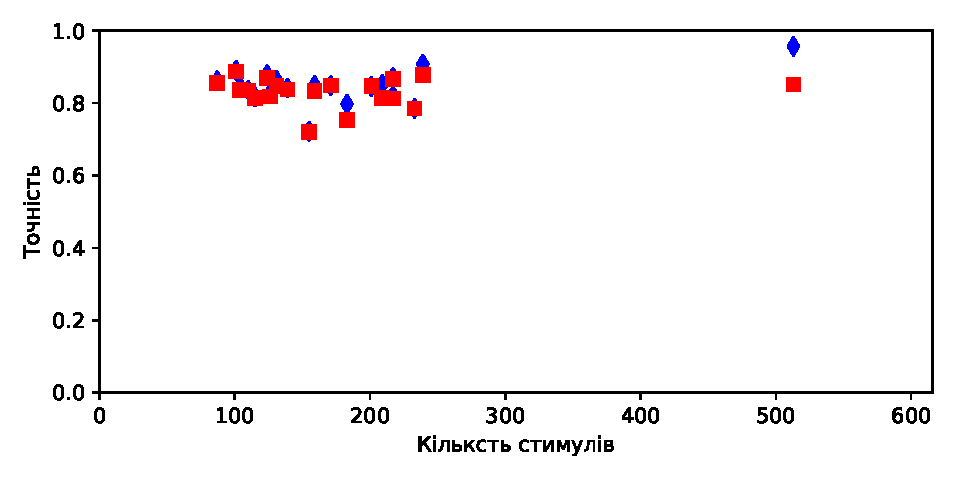
\includegraphics[width=\linewidth]{accuracy_distribution_data1_cnn}}
	\caption{Розподіл точності (червоні квадрати) та F-міри (сині ромби) за кількістю голосових зразків при моделюванні контекстів різними методами}
	\label{img:accuracy_distribution_data1}
\end{figure}

З матриці помилок (confusion matrix) \cite{Stehman_1997} моделювання тестового контексту методом інтелектуальних рефлекторних систем (рис. \ref{img:confusion_matrix_data1_irs13_context_21} та \ref{img:confusion_matrix_data1_irs24_context_21}), ми можемо бачити, що рівень розпізнавання близький до 50\% досягається за рахунок того, що всі реакції в контексті розпізнаються, як реакція №2. Оскільки вона представлена найбільшою кількістю зразків, точність досягає відносно високих значень при насправді низькій якості моделі.

\begin{figure}[!t]
	\centering
	\subbottom[Метод ІРС розміром 1--3 \label{img:confusion_matrix_data1_irs13_context_21}]{%
		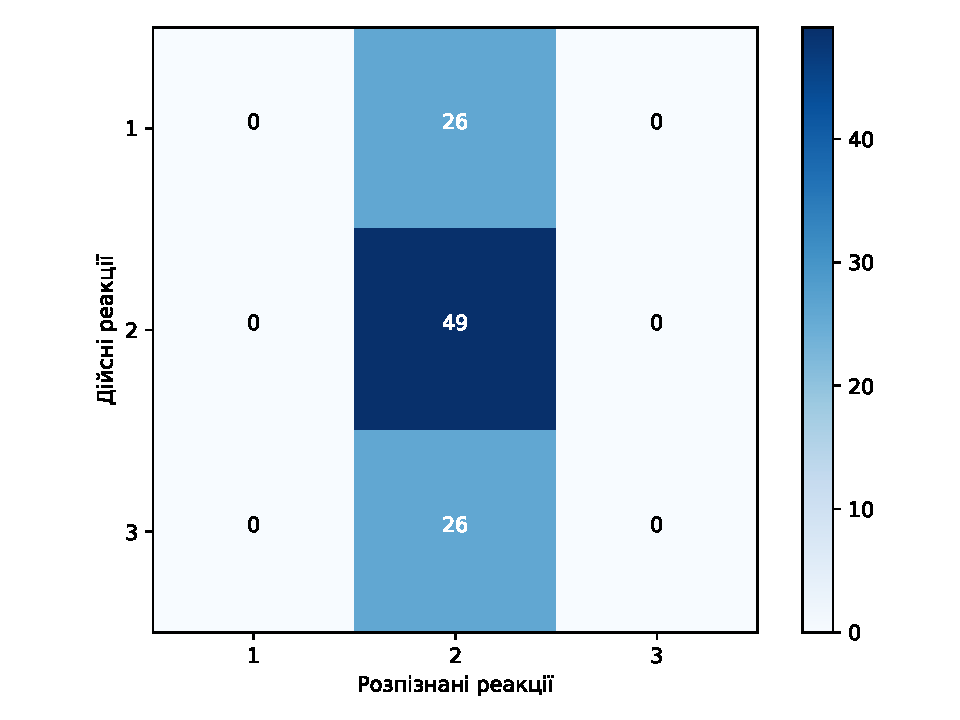
\includegraphics[width=.9\linewidth]{confusion_matrix_data1_irs13_context_21}}
	\subbottom[Метод ІРС розміром 2--4 \label{img:confusion_matrix_data1_irs24_context_21}]{%
		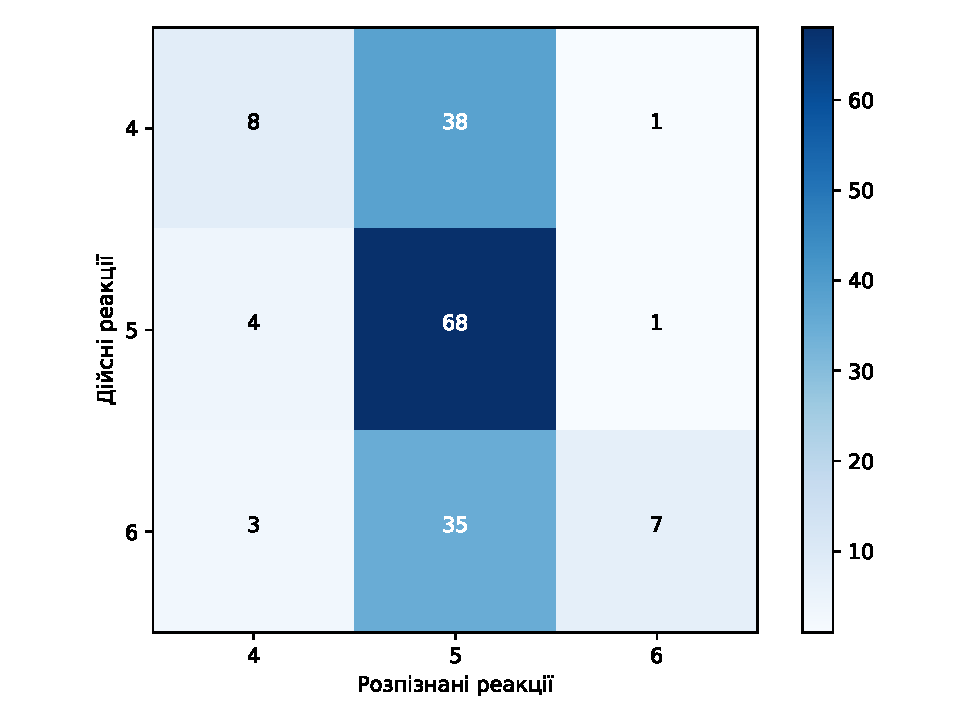
\includegraphics[width=.9\linewidth]{confusion_matrix_data1_irs24_context_13}}
	\subbottom[Метод ЗНМ \label{img:confusion_matrix_data1_cnn_context_21}]{%
		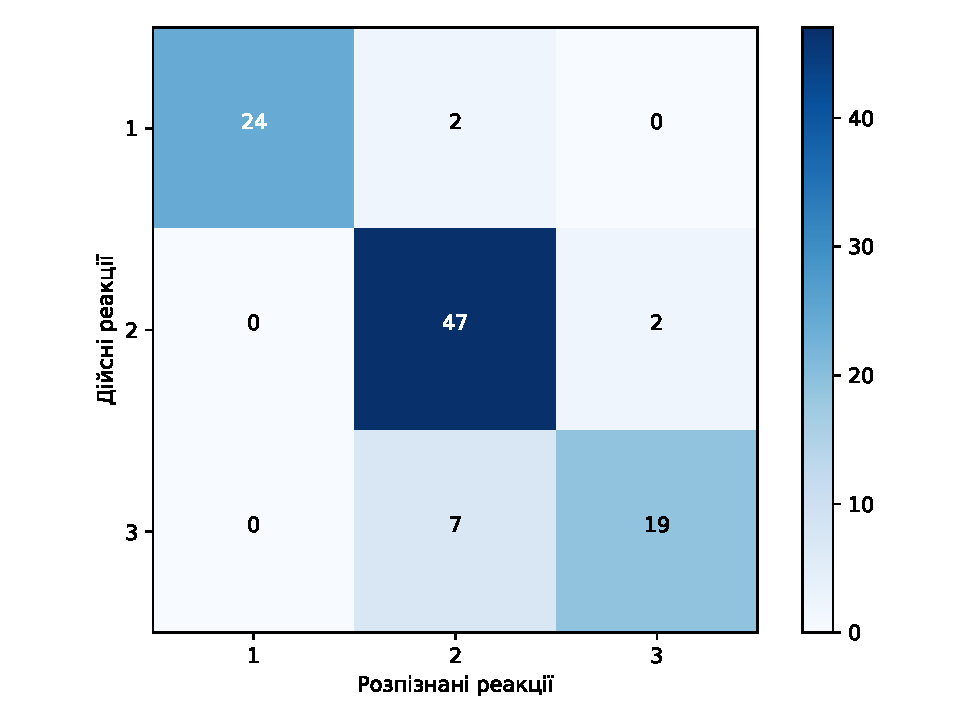
\includegraphics[width=.9\linewidth]{confusion_matrix_data1_cnn_context_21}}
	
	\caption{Порівняння матриць помилок трьох різних методів (а, б, в) розпізнавання по реакціях для тестового контексту першого набору даних}
	\label{img:confusion_matrix_data1_context_21}
\end{figure}

Дослідивши матриці помилок моделювання інших контексів методом інтелектуальних рефлекторних систем було виявлено, що моделі всіх контекстів в тій чи іншій мірі схильні до подібних помилок. Найменш схильними виявилися моделі контекстів 14, 16, 18 та 19, але за таблицею ми можемо бачити, що значення точності для цих контекстів менші за точність моделей для 13-го та тестового контекстів, де всі реакції були розпізнані як одна й та ж сама (рис. \ref{img:confusion_matrix_data1_irs13_context_21}).

Як кращі міри якості класифікаційної моделі для незбалансованих вибірок зазвичай використовують прецизійність (precision) та повноту (recall), які у випадку небінарної класифікації можуть бути визначені лише для певного класу, а не для моделі в цілому \cite{Powers_2011}. Для оцінки якості моделі було використано середні показники прецизійності та повноти по всім реакціям, що можуть бути визначені по формулам:

\begin{equation}
\label{eq:рrecision}
P=\frac{1}{n}\sum\limits_i\frac{TP_i}{TP_i+FP_i};
\end{equation}

\begin{equation}
\label{eq:recall}
R=\frac{1}{n}\sum\limits_i\frac{TP_i}{TP_i+FN_i},
\end{equation}

де $P$ --- середня прецизійність, $R$ --- середня повнота, $n$ --- кількість класів, $TP_i$ --- кількість вірно розпізнаних (True positive) зразків реакції $i$, $FP_i$ --- кількість зразків хибно розпізнаних (False positive) як реакція $i$, a $FN_i$ -- кількість зразків реакції $i$, хибно розпізнаних (False negative) як інша реакція.

Оскільки прецизійність показує лише помилки першого роду, а повнота лише помилки другого роду, існує узагальнена F-міра (F1, F-score) \cite{Powers_2011,Sasaki_2007}, що враховує обидва типи помилок як середньо-гармонічне, та може бути визначена за формулою:

\begin{equation}
\label{eq:f1}
F_1 = 2 \cdot \frac{P \cdot R}{P + R},
\end{equation}

де $F_1$ --- F-міра, $P$ --- прецизійність а $R$ --- повнота.

Дослідивши значення F-міри з таблиці \ref{tbl:total_data1_irs13} ми бачимо, що саме моделі контекстів 14, 16, 18 та 19, які виглядають найкраще на матрицях помилок, мають одні з найбільших значень F-міри, та порівняні зі значеннями моделей контекстів 1 та 2, що складаються лише з двох реакцій. Моделювання методом ІРС з розміром N-грам 2–4 (табл. \ref{tbl:total_data1_irs24}) показало схожі результати і дало невеликий приріст. якості розпізнавання, але цієї якості все одно недостатньо для практичного застосування моделі.

Метод згорткових нейронних мереж показав кращий результат. З таблиці \ref{tbl:total_data1_cnn} видно, що значення F-міри не набагато нижчі за точність, з чого можна зробити висновок, що ця модель краще працює з незбалансованими вибірками.

Для розрахунку показників у таблицях \ref{tbl:total_data1_irs13}--\ref{tbl:total_data1_cnn} використовувався метод кросс-валідації \cite{Kohavi_1995} з розбиттям повної вибірки на 5 рівних випадкових частин. Таким чином моделювання проводилося 5 разів, так, щоб кожна з 5 частин один раз була використана як тестова вибірка, а 4 інших частини в кожному моделюванні складали навчальну вибірку. Саме комбінація результатів на тестовій вибірці з 5-ти моделювань і була використана для розрахунку метрик в таблицях.

Розрахунок метрик на тестових вибірках показував точність розпізнавання від 90\% до 100\%, це свідчить про ефект перенавчання системи. Одним зі способів вирішення проблеми перенавчання є збільшення кількості даних. Було висунуто гіпотезу про низьку якість розпізнавання в зв’язку з недостатньою кількістю вхідних даних.

Отже, було вирішено провести другий етап дослідження, для якого було необхідно зібрати більшу кількість голосових даних. Для перевірки гіпотези вирішено зібрати голосові зразки лише для одного тестового контексту.

Додаткові голосові дані зібрано для одного контексту: 1 пристрій, 1 диктор (чоловік), 37 варіантів стимулів, 3 реакції у контексті, тобто 938 зразків.

Результати моделювання другого набору даних трьома різними методами ми можемо бачити в таблиці \ref{tbl:total_data2_irs13}, а матриці помилок зображено на рисунку \ref{img:confusion_matrix_data2_context_21}.

\begin{mytable}{ | c | c | c | c | }%
	{Порівняння якості розпізнавання другого набору даних різними методами}%
	{\label{tbl:total_data2_irs13}}%
	{ Показник & ІРС 1--3 & ІРС 2--4 & ЗНМ }		
	
	Точність розпізнання & 0.258 & 0.598 & 0.935 \\
	\hline
	Середня прецизійність & 0.226 & 0.636 & 0.939 \\
	\hline
	Середня повнота & 0.238 & 0.579 & 0.935 \\
	\hline
	Середня F-міра & 0.217 & 0.583 & 0.937 \\
	\hline
	Кількість & 925 & 925 & 925 \\
\end{mytable}

\begin{figure}[ht!]
	\centering
	\subbottom[Метод ІРС розміром 1--3 \label{img:confusion_matrix_data2_irs13_context_21}]{%
		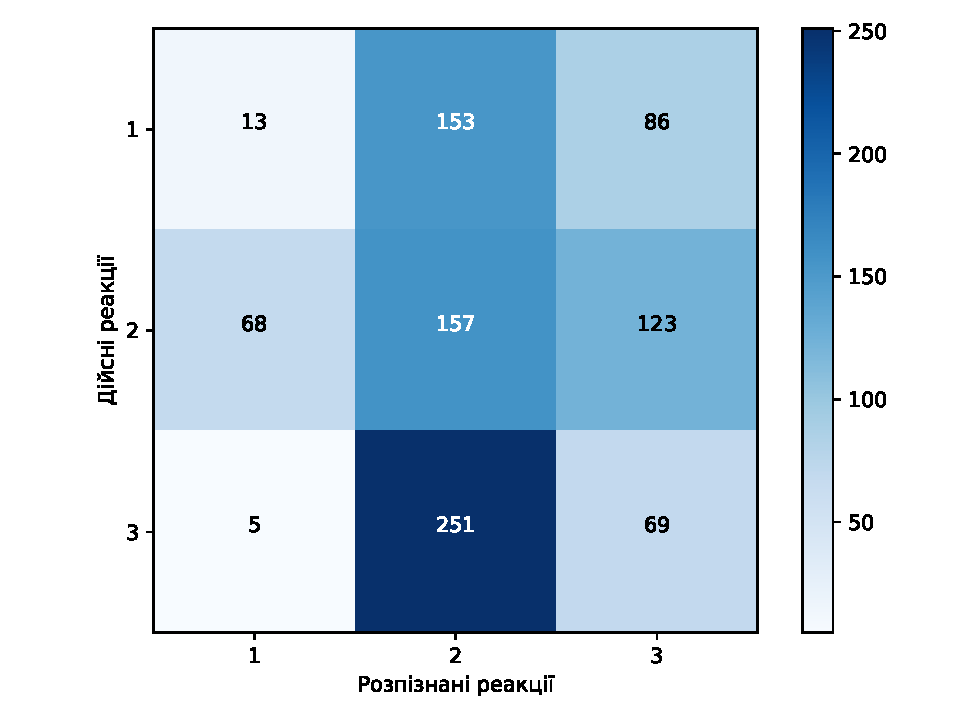
\includegraphics[width=.9\linewidth]{confusion_matrix_data2_irs13_context_21}}
	\subbottom[Метод ІРС розміром 2--4 \label{img:confusion_matrix_data2_irs24_context_21}]{%
		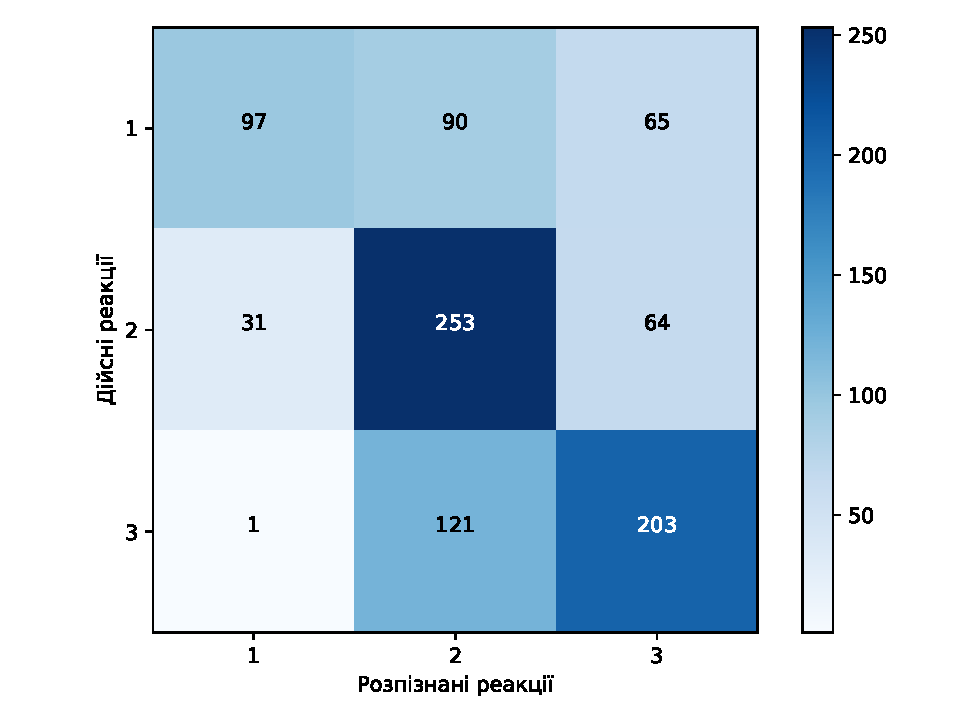
\includegraphics[width=.9\linewidth]{confusion_matrix_data2_irs24_context_21}}
	\subbottom[Метод ЗНМ \label{img:confusion_matrix_data2_cnn_context_21}]{%
		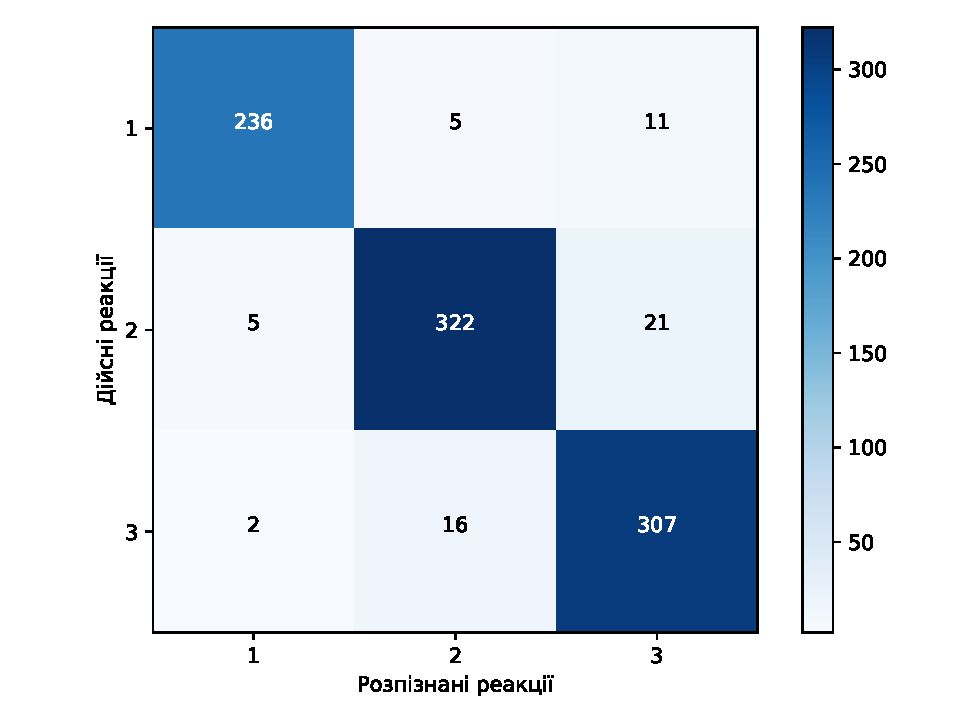
\includegraphics[width=.9\linewidth]{confusion_matrix_data2_cnn_context_21}}
	
	\caption{Порівняння матриць помилок трьох різних методів (а, б, в) розпізнавання по реакціях для тестового контексту другого набору даних}
	\label{img:confusion_matrix_data2_context_21}
\end{figure}

З результатів моделювання можна бачити, що збільшення кількості вхідних даних безумовно покращило якість розпізнавання, для всіх методів. Моделювання інтелектуальними рефлекторними системами для одного контексту з великою вибіркою даних дало майже 60\% точності та значення F-міри 0.58. З матриці помилок (рис. \ref{img:confusion_matrix_data2_irs24_context_21}) не має явного переважання певної реакції над іншими. На жаль, отриманих значень точності досі недостатньо для успішного використання моделі на практиці. 

Моделювання методом згорткових нейронних мереж дало трохи більше 90\% точності та відповідне значення F-міри. Така точність є достатньою для практичного застосування, отже можна зробити висновок, що за даних умов дуальна система класифікації фонемної репрезентації голосових команд працює краще з використанням методу згорткових нейронних мереж для побудови моделі формалізації голосової інформації в системах диспетчеризації автотранспорту.

\section{Обговорення результатів}

Порівняння різних метрик ефективності моделей небінарної класифікації показало, що для моделей високої якості, а також у випадках збалансованих вибірок даних, всі метрики показують схожі значення ефективності. Але у випадках моделей, які негативно реагують на незбалансованість вибірки, F-міра оцінює модель набагато точніше.

Було проведено 2 етапи моделювання. На первинному етапі зібрано голосові дані 23 дикторів, у середньому по 45 зразків на реакцію. Результати моделювання обома методами показали точність не вищу за 50\%, що є недостатньою для практичного застосування. Точність класифікації на навчальних даних була близькою до 100\%, що свідчить про перенавчання.

На основі цього було висунуто гіпотезу про недостатню кількість голосових даних, тому на другому етапі зібрано в середньому 310 голосових зразків для кожної з 3-х реакцій простого контексту.  Моделювання методом інтелектуальних рефлекторних систем показало точність біля 60\%, що також є недостатнім, а методом згорткових нейронних мереж — трохи більше за 90\%, що є прийнятним.

З цього можна бачити, що за даних умов, ефективність методу згорткових нейронних мереж вища за метод інтелектуальних рефлекторних систем більш ніж на 30\%. Ці результати викликають певний подив, оскільки в попередніх дослідженнях \cite{Egorchenkov_2016,Teslia_2014,Teslia_2013} метод інтелектуальних рефлекторних систем давав набагато кращі результати. Візуально дослідивши фонемну репрезентацію даних, ми помітили сильну зашумленість фонемних даних, хоча в звукових файлах рівень шуму був нижчим. Одне з можливих пояснень цього полягає в тому, що фонемний стенограф не був налаштований на використання мікрофону в мобільному телефоні, частотні показники якого можуть вносити перешкоди в роботу системи.  

Тобто, висунуто наступну гіпотезу про недостатню якість звукового запису та високий рівень шумів як перешкоди ефективності моделі формалізації. Перспективою подальшого розвитку є проведення наступного етапу дослідження, для якого необхідно зібрати нову вибірку даних з використанням більш якісного зовнішнього мікрофона. Крім того, для усунення впливу незбалансованої вибірки даних, пропонується зібрати рівну кількість записів для кожної реакції з дерева сценаріїв голосової взаємодії.

\section{Висновки}

Перевірка моделювання розпізнавання команд на основі ітеративного процесу збору даних та введення нових критеріїв оцінки, якщо попередні не дали достатньої точності оцінювання, може забезпечити процес порівняння ефективності різних методів класифікації в дуальній моделі формалізації голосової взаємодії.

Доцільно використовувати набір метрик оцінки ефективності моделей класифікації, що обов’язково має включати крім оцінки точності ще робастні метрики для незбалансованої вибірки (такі, як прецизійність, повноту, F-міру) або візуальний аналіз матриць помилок. 

Досягнуто прийнятний для практичного використання рівень точності в моделі, побудованої методом згорткових нейронних мереж при другій ітерації моделювання з достатньою кількістю навчальних даних.

Для підтвердження ефективності методу інтелектуальних рефлекторних систем двох ітерацій виявилося недостатньо, висунуто гіпотезу про недостатню якість звукового запису та високий рівень шумів як перешкоди ефективності моделі формалізації, окреслено перспективи проведення наступного етапу дослідження.

Загалом за результатами проведеної роботи підтверджено ефективність рефлекторної системи голосового управління, яка складається з фонемного стенографа і ядра класифікації, і здатна на практиці  визначати зміст та керуючий вплив отриманого набору фонем без перетворення голосової інформації в текстову форму. 


